\documentclass{article}
\usepackage{caption}
\usepackage{subcaption}
\usepackage{graphicx}
\usepackage{tikz}
\usepackage{tikzsymbols}
\usetikzlibrary{calc,patterns,shapes.geometric}
\usepackage{float}
\usepackage{pdflscape}


\def\centerarc[#1](#2)(#3:#4:#5){\draw[#1] ($(#2)+({#5*cos(#3)},{#5*sin(#3)})$) arc (#3:#4:#5);}

\pagestyle{empty}
\begin{document}
	\centering
	\begin{figure}[H]
		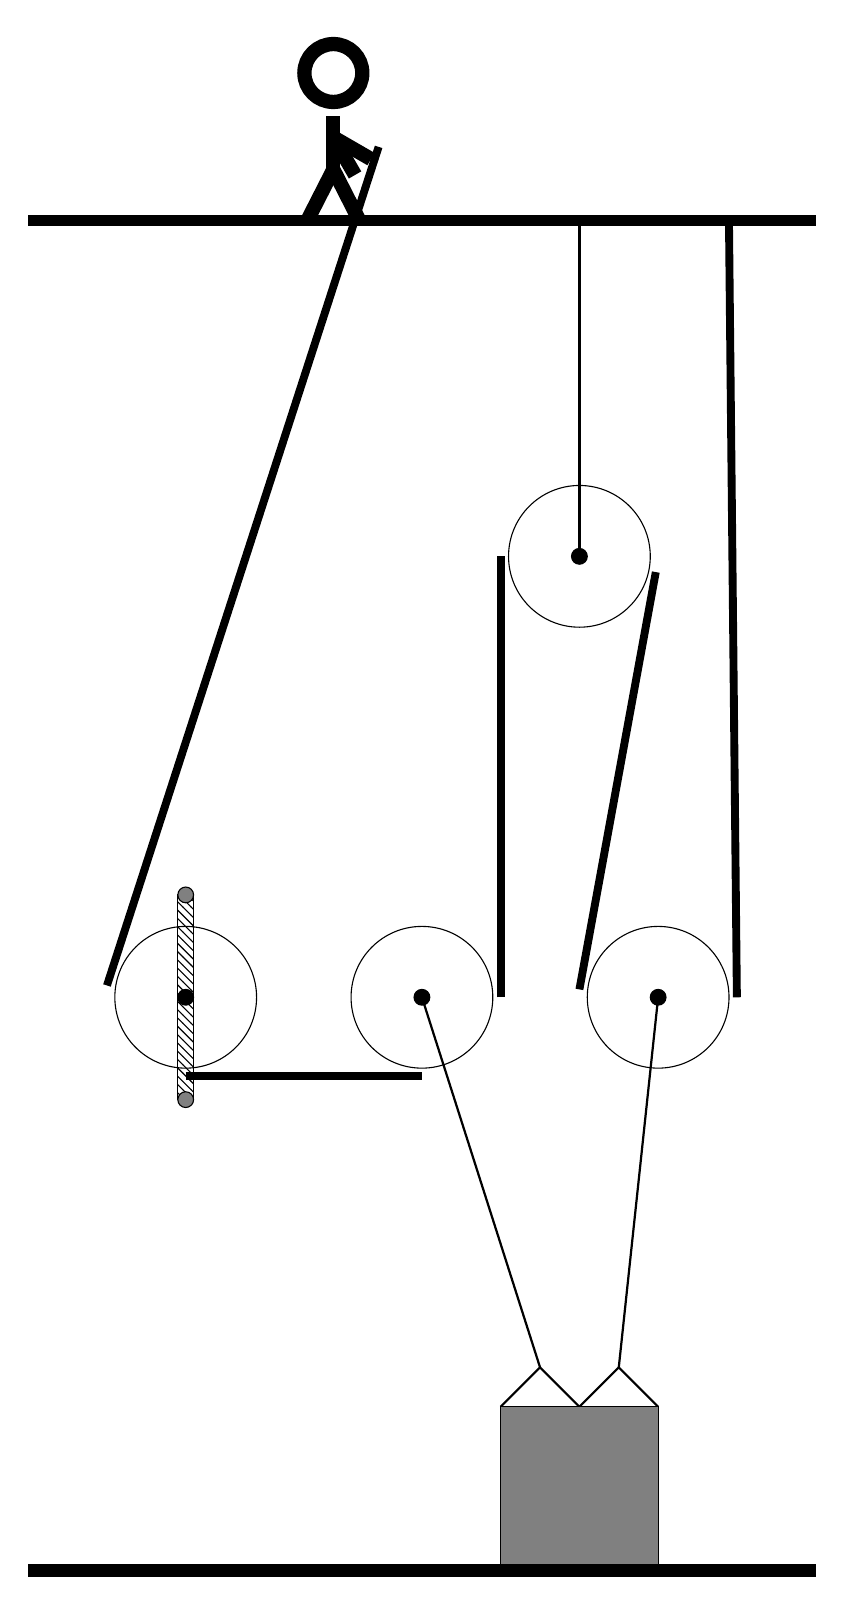
\begin{tikzpicture}
			%%%%% START %%%%%
			\def\a{14}
			\def\radlg{\radrp-0.1}
			\def\radrp{1}
			\def\radsm{0.1}
			\def\xone{1}
			\def\yone{\a*0.3}
			\def\xtwo{\xone+2}
			\def\ytwo{\a*0.7}
			\def\xthree{\xone+3}
			\def\ythree{\a*0.3}
			\def\dx{-0.05}
			\def\dy{\a*1.5}
			\def\hlen{-3}
			\def\width{1mm}
			\def\ywallone{\yone}
			\def\xwallone{\xone-3}
			\def\bump{0.3}
			
			\draw[fill=black] (-4,\a) rectangle (6,\a+0.125);
			
			\draw (\xone,\yone) circle (\radlg);
			\draw[fill=black] (\xone,\yone) circle (\radsm);
			
			\draw (\xtwo,\ytwo) circle (\radlg);
			\draw[fill=black] (\xtwo,\ytwo) circle (\radsm);
			\draw[thick] (\xtwo,\ytwo) -- (\xtwo,\a);
			
			\draw (\xthree,\ythree) circle (\radlg);
			\draw[fill=black] (\xthree,\ythree) circle (\radsm);
			
			\draw[thick] (\xthree,\ythree) -- (\xtwo+0.5,\hlen+2.5);
			\draw[thick] (\xone,\yone) -- (\xtwo-0.5,\hlen+2.5);
			\draw[thick]  (\xtwo-1,\hlen+2) -- (\xtwo-0.5,\hlen+2.5) -- (\xtwo,\hlen+2);
			\draw[thick]  (\xtwo,\hlen+2) -- (\xtwo+0.5,\hlen+2.5) -- (\xtwo+1,\hlen+2);
			\draw[fill=black!50] (\xtwo-1,\hlen+2) rectangle (\xtwo+1,\hlen);
			
			% wall polly one
			\draw[pattern=north west lines, pattern color=black] (\xwallone-0.1,\ywallone+\radrp+\bump) rectangle (\xwallone+0.1,\ywallone-\radrp-\bump); 
			\draw[fill=black!50] (\xwallone,\ywallone+\radrp+\bump) circle (\radsm);
			\draw[fill=black!50] (\xwallone,\ywallone-\radrp-\bump) circle (\radsm);
			
			\draw (\xwallone,\ywallone) circle (\radlg);
			\draw[fill=black] (\xwallone,\ywallone) circle (\radsm);
			

			
			
			
			\draw[line width=\width] (\dx+0.5,\a+1) -- (\xwallone-\radrp*1, \ywallone+\radrp*0.15);
			\centerarc[line width=\width](\xwallone,\ywallone)(160:270:\radrp);
			
			\draw[line width=\width](\xwallone,\ywallone-\radrp) -- (\xone,\yone - \radrp); 
			\centerarc[line width=\width](\xone,\yone)(270:360:\radrp);
			\draw[line width=\width] (\xone+\radrp,\yone) -- (\xtwo-\radrp,\ytwo);
			\centerarc[line width=\width](\xtwo,\ytwo)(-20:180:\radrp);
			\draw[line width=\width](\xtwo+\radrp*0.97,\ytwo-\radrp*0.2) -- (\xthree-\radrp*1,\ythree+\radrp*0.1);
		\centerarc[line width=\width](\xthree,\ythree)(160:360:\radrp);
			\draw[line width=\width](\xthree+\radrp,\ythree) -- (\xthree+\radrp-0.1,\a);
			
			\node at (-0.07, \a+1.2) {\Strichmaxerl[10][120][-30]};
			
			\draw[fill=black] (-4,-3) rectangle (6,-3.15);
			%%%%% END %%%%%
		\end{tikzpicture}
	\end{figure}
	
\end{document}